
% SEP 2012 Group 13
% Software Requirements Document (SRS)
%
\documentclass[11pt, a4paper]{report}
\usepackage{graphicx}
\usepackage{pdfpages}
\usepackage{fullpage}
\usepackage{url}
\pagestyle{headings}

%%% page parameters
\headsep = 25pt
\begin{document}
\oddsidemargin -0.5 cm
\evensidemargin -0.5 cm
\textwidth 15 cm
\topmargin -1.2 cm
\textheight 25 cm
\begin{center}

\includegraphics[scale=1.5]{./UniLogo}\\[1cm]    
\textbf{\Huge \bfseries User Manual}\\[1.5cm]
\textbf{\huge for}\\[0.5cm]


% Title
\textbf{ \huge Archaeology Robot }\\[0.3cm]
\textbf{ \huge Team 13 }\\[2cm]


\begin{tabular}{ |c | p{2cm} |}
	\hline
Yufeng Bai 1600095 & \\[.5cm] \hline
Jun Chen 1206265 & \\[.5cm] \hline
Dawei Geng 1219181 & \\[.5cm] \hline
Yunyao Yao 1203525 & \\[.5cm] \hline
Shikai Li 1214223 & \\[.5cm] \hline
Quang Khoi Nguyen 1187070  & \\[.5cm] \hline
Yatong Zhou 1204471 & \\[.5cm] \hline
\end{tabular}


\vfill

% Bottom of the page
Version 1.0 \\ [0.2cm]
{\large \today}

\end{center}


\tableofcontents



% Version History %

% IMPORTANT %
% Whenever you make a change to this document you MUST put an entry in below
% Must conform to firstName lastName &  date & discription \\ \hline


\clearpage
\section*{Revision History}
\begin{tabular}{| l | l | l | l | }
\hline
Name      		&	Date        	&	Reason For Changes								&	Version			\\ \hline
Dawei Geng      &	21 Aug 2012    	&	basic framework of the SPMP and Chapter 1		&	0.1				\\ \hline
Dawei Geng      &	23 Aug 2012    	&	Chapter 3 \& Section 4.1						&	0.19			\\ \hline
Dawei Geng      &	24 Aug 2012     &	Section 4.2.1 \& 4.2.2							&	0.2				\\ \hline
Dawei Geng     	&	25 Aug 2012     &	Chapter 5										&	0.3				\\ \hline
Jun Chen		&	25 Aug 2012		&	Spelling \& grammar check , error fix			&	0.31			\\ \hline
Yufeng Bai      &	27 Aug 2012		&	Chapter 7										&	0.32			\\ \hline
Yaong Zhou		&	29 Aug 2012		&	Error Fix and Grammer Check						&	0.33			\\ \hline
Dawei Geng      &	01 Sep 2012     &	5.1.4 \& Appendix edit \& bug fix				&	0.4				\\ \hline
Jun Chen     	&	02 Sep 2012     &   Grammar Check \& Fixing Layout Error			&	0.4				\\ \hline
Dawei Geng     	&	02 Sep 2012     &	Re-fix Layout Error	\&  						&	0.45			\\ \hline
Khoi Nguyen		&	04 Oct 2012		&	Review, Final Version							&	0.46	\\ \hline
Yufeng Bai	&	07 October	&	Fixing chapter 6									&	0.47\\ \hline
Khoi Nguyen     &	07 Oct 2012    	&	Testing plan									&	0.48			\\ \hline
Jun Chen     		&	09 Oct 2012         	&Review, fixing chapter 7-8									&	0.49			\\ \hline
Jun Chen     		&	10 Oct 2012         	&layout fixing									&	0.50			\\ \hline
%Name      		&	Date        	&	Reason For Changes								&	Version			\\ \hline
%Name      		&	Date        	&	Reason For Changes								&	Version			\\ \hline
%Name      		&	Date        	&	Reason For Changes								&	Version			\\ \hline





\end{tabular}
\clearpage

% Introduction %

\chapter{Introduction}

\section{Purpose and Scope}
This document aims to provide information that is required to manage the overall design, implementation and maintenance of the project of archaeology robot. \\ \\
This document will be divided into seven parts, including the Introduction, Definitions, Project organization, Risk management plan, Process model, Work plan, and the Supporting plans.

\begin{enumerate}
	\item \textbf{Project organization} describes the responsibilities for each member of the team and the reason behind this arrangement.
	\item \textbf{Risk management} outlines the risks may be found during the development of the project, also includes risk analysis and the processes and strategies for the team members to control or overcome these risks.
	\item \textbf{Process model} describes the process model will be used throughout the whole development. Including the critical paths and major stages taken in the development. Rational behind this choice will be provided, along with the advantages and disadvantages of this process model. 
	\item \textbf{Work plan} includes the tasks will be done to deliver the product, and the milestones that the team will be meeting during the development. Work plan will also include the duration of the tasks and the allocation of the resources to these tasks.
	\item \textbf{Supporting plans} outlines the configuration management plan, the documentation plan, and quality assurance plan.
\end{enumerate}


\section{Assumptions and constraints}
This project will be developed under such assumptions and constraints:
\begin{enumerate}
	\item Every group member has a laptop/desktop with LeJos Driver installed.
	\item Every member's computer needs to install JRE and SDK.
	\item Every member's computer needs to have access to Internet and group's SVN repository.
	\item A Bluetooth connection can be created between the robot and every team member's PC.
	\item A Lego Mindstorm NXT robot will be used in this project. 
	\item This project has a duration of 11 weeks.
	\item Every member have the knowledge or skills to carry out the tasks which
are assigned to them.
	\item This project requires at least 10 hours per week workload for every team member.
\end{enumerate}

\section{Project deliverables}
The following items will be delivered to the client throughout the development of this project.
\begin{enumerate}
	\item Team Poster
	\item Software Requirement Specification (SRS)
	\item Software Project Management Plan (SPMP)
	\item Software Design Document (SDD)
	\item Testing Report
	\item User Manual
	\item Project Milestone Demonstration
	\item Final Project Demonstration
\end{enumerate}


\section{Evolution of the plan}
This plan will be made by the team during the requirements elicitation and system design. The plan shall be made by gathering the feedback from the clients, and negotiation with clients about the milestones. In the software developing stage, the plan shall be changed under the circumstances:
\begin{enumerate}
	\item Requirements changed by the clients
	\item A defect of the plan was found
	\item Other unexpected situations such as a team member is missing. \\ \\
\end{enumerate} 
At the planning stage, clients shall be able to change or raise requirements at anytime. However once the plan have been made and the team enter the developing stage, if a change is needed, the clients shall negotiate with the project manager along with team members to achieve the changes. \\ \\
If a defect of the plan was found, it will be raised in the group meetings and the whole team shall discuss and respond to the possible changes.\\ \\
Other unexpected situations such as team member missing , will lead to the whole team meeting with the client to discuss how to overcome such situations. 


\pagebreak


\chapter{References}
\begin{enumerate}
\item The project description by the client:
http://forums.cs.adelaide.edu.au/forum/SEP-S2-2012/ProjectDescription2012.pdf
\item The SPMP template:
http://forums.cs.adelaide.edu.au/forum/SEP-S2-2012/SPMP.pdf
\item The lecture notes:
http://forums.cs.adelaide.edu.au/course/view.php?id=452
\item JUnit:
http://www.junit.org
\item Minutes of client meeting
\item Minutes of Internal meeting
\end{enumerate}

\pagebreak


\chapter{Definitions}
\begin{tabular}{| l | l | }
\hline
Acronym      		&	Definition       											\\ \hline
Gantt Chart      	& 	A type of bar chart, which illustrates a project schedule.	\\ \hline
GUI					& 	Graphic User Interface 										\\ \hline
{\LaTeX}			&	Document markup language for {\TeX} typesetting program 	\\ \hline
QA 					&	Quality assurance 											\\ \hline
SEP					&	Software engineering project								\\ \hline
SPMP				&	Software Project Management Plan							\\ \hline
SRS					&	Software Requirements Specification							\\ \hline
SVN					&	Subversion repository										\\ \hline
{\TeX} 				&	A system for computer typesetting. Used by {\LaTeX}			\\ \hline
XML					& 	Extensible Markup language 									\\ \hline
\end{tabular}

\pagebreak


\chapter{Project Organization}

\section{Roles and responsibilities}
The team for this project is made up of seven members, which will be divided into project manager, documentation manager, QA manager, developer, and QA engineer. Each team member will have one or two specific role, however, a team member will be limited to his role. However, he or she is free to help others. In this chapter, each role's main responsibilities will be explained and the team members who are assigned to the role.

\paragraph{Role: } Project Manager
\paragraph{Member: } Dawei Geng
\paragraph{Responsibilities: }
\begin{enumerate}
	\item  Ensuring the goal of this project will be achieved to the client's satisfaction.
	\item  Developing project milestones and overall project plan.
	\item  Organizing team members and their roles to fulfill the project needs.
	\item  Ensuring the project runs according to the milestones and project plan.
\end{enumerate}
\paragraph{Rational: \\} 
Being a project manager requires leadership, team spirit, problem solving skills, and much more. Dawei Geng have worked in groups and stood out when a plan is needed for the project. In case of leadership, team working, and project planning, Dawei Geng did a very nice job. 

\paragraph{Role: } Documentation Manager
\paragraph{Member: } Yufeng Bai
\paragraph{Responsibilities: }
\begin{enumerate}
	\item  Organizing the project's documents and keeping documents up to date.
	\item  Helping project manager organize meeting agendas and minutes.
	\item  Keep track of the SVN repository.
	\item  Spelling and grammar checking.
\end{enumerate}
\paragraph{Rational: \\}
As a documentation manager Yufeng Bai must take full responsible for all the document changes and delivery, this job requires responsibility and professional English skills to manage the documents. Yufeng Bai has an excellent written skills to meet the demand of the role.

\paragraph{Role: } QA Manager
\paragraph{Member: } Khoi Nguyen
\paragraph{Responsibilities: }
\begin{enumerate}
	\item  Planning, organizing all the test-related tasks
	\item  Setting up the test strategies
	\item  Reviewing the code and test plans with QA engineers.
\end{enumerate}
\paragraph{Rational: \\}
Besides of being a good QA engineer, the role requires additional skills such as communication, creativity and team management. Khoi can be a qualified QA manager.

\paragraph{Role: } Main Developer
\paragraph{Member: } Khoi Nguyen, Yatong Zhou, and Yaoyun Yao
\paragraph{Responsibilities: }
\begin{enumerate}
	\item  Developing the software of the robot and the host machine based on the requirements.
	\item  Following the milestones and project plan. 
	\item  Delivering high quality code and software.
\end{enumerate}
\paragraph{Rational: \\}


\paragraph{Role: } GUI Developer
\paragraph{Member: } Yatong Zhou and Shikai Li
\paragraph{Responsibilities: }
\begin{enumerate}
	\item  Developing the graphical user interface.
	\item  Providing test GUI to the main developers.
\end{enumerate}
\paragraph{Rational: \\}
Yatong Zhou and Shikai Li have high level of developing graphic user interface using Java and understand the concept of presenting the useful information to the user in an elegant and efficient way.

\paragraph{Role: } QA Engineer
\paragraph{Member: } Shikai Li and Jun Chen
\paragraph{Responsibilities: }
\begin{enumerate}
	\item  Being responsible for all the te st-related tasks.
	\item  Following the testing plans.
	\item  Code reviewing.
	\item  Writing test report.
\end{enumerate}
\paragraph{Rational: \\}
Sikhai Li and Jun Chen are excelled at problem solving and trouble shooting. 
At the same time, both of them are patient, which is important in this kind of role.

\chapter{Risk management plan}
\subsection{Purpose}
Risk is defined as the events which occurred during the development of the project, and could have positive or negative impact to the development. A certain risk may be caused by one or more causes and may have one or more impacts. This plan document's processes, tools, and procedures will be taken to manage or control the events which could have negative effect to the project. It will include:
\begin{enumerate}
	\item Foreseeable Risks Identification.
	\item Risk's Impact Prediction.
	\item Risk's Likelihood Prediction.
	\item Risk Response Plan.
\end{enumerate}
As summary, this plan will list each identified risk based on the priority: the likelihood of certain risk and the impact of it. A plan in which to reduce the risk from occurring will be suggested.

\subsection{Risk Assessment}
This section will list each identified risk and give it a ID initialed with letter "R". The probability and the impact of each risk will be represented as the category of "Low", "Medium", and "High". \\
	\paragraph{R001: Team member unable to work} \hspace{1cm} \textbf{Probability: }High\hspace{1cm}   \textbf{Impact: }Medium
	\paragraph{Description}As a three months project, team members who get sick or have personal affair will be unable to perform enough in the project. Therefore, someone else in the team will have to double the workload.
	\paragraph{Indicator}A team member does not attend lectures and meetings with no work submitted for over one week or call for absence.
	\paragraph{Mitigation}All the work shall be evenly assigned. Every group member needs to pay attention to his/her health condition.
	\paragraph{Response Plan}Divide missing team member's workload into parts and assign them to other group members who are available to do it. \\
	\paragraph{Category} Project risk

	\paragraph{R002: Conflict between group members} \hspace{1cm} \textbf{Probability: }Medium\hspace{1cm}   \textbf{Impact: }Low
	\paragraph{Description}Team members have arguments or conflicts about the development or design.
	\paragraph{Indicator}Team members are arguing or refusing to complete their tasks.
	\paragraph{Mitigation}Every issue regarding the design or implementation of this project will be discussed in the internal meeting or client meeting. The solution of this issue shall satisfy every team member.
	\paragraph{Response Plan}An emergency meeting will be held within the group to discuss the controversial issue. A voting process may be held.\\
	\paragraph{Category} Project risk
	
	\paragraph{R003: Fail or late delivery} \hspace{1cm} \textbf{Probability: }Medium\hspace{1cm}   \textbf{Impact: }Medium
	\paragraph{Description}Team member's deliverable is not on time.
	\paragraph{Indicator}Late commits or no commit over the preset deliverable deadline.
	\paragraph{Mitigation}Ensure team members have proper workload, understanding of the importance of delivery on time. 
	\paragraph{Response Plan}Other team members shall help the team member who fail or late of delivery to make the project follow the project plan. \\
	\paragraph{Category} Project risk
%\pagebreak

	\paragraph{R004: Lack of contribution} \hspace{1cm} \textbf{Probability: }Medium\hspace{1cm}   \textbf{Impact: }Medium
	\paragraph{Description}Team member fail to contribute as much as others in the team.
	\paragraph{Indicator}Team member has no or lack of submission to the SVN repository. 
	\paragraph{Mitigation}Project manager shall separate the workload properly.
	\paragraph{Response Plan}When this problem is found, team leader or project manager shall "rebalance" the workload. \\
	\paragraph{Category} Project risk
	
	\paragraph{R005: Team member leave the project permanently} \hspace{1cm} \textbf{Probability: }Low\hspace{1cm}   \textbf{Impact: }High
	\paragraph{Description}Due to possible reasons, one team member may withdraw from the course. He/she leaves the project permanently.
	\paragraph{Indicator}The team member notifies the team with certain intention.
	\paragraph{Mitigation}The manager should ensure that there is no critical important job that can be done by just one person.
	\paragraph{Response Plan}An emergency meeting will be held within the group immediately.  The leaving member's original unfinished task will be reallocated to the remaining members.\\
	\paragraph{Category} Project risk
	
	\paragraph{R006: Project file lost} \hspace{1cm} \textbf{Probability: }Low\hspace{1cm}   \textbf{Impact: }High
	\paragraph{Description}Data or files may lose caused by computer damage.
	\paragraph{Indicator}Team member's hardware has problems. 
	\paragraph{Mitigation}Every team member shall keep committing to the SVN repository regularly.
	\paragraph{Response Plan}Data rescue methods will be carried out in order to retrieve the missing data or files.\\
	\paragraph{Category} Product risk
	
	\paragraph{R007: SVN failure} \hspace{1cm} \textbf{Probability: }Low\hspace{1cm}   \textbf{Impact: }High
	\paragraph{Description}The team's SVN repository is "offline" or does not work correctly.
	\paragraph{Indicator}Grope member continuously fail to commit or update changes from the SVN repository. In addition, system failed or other error messages are received continuously.
	\paragraph{Mitigation}A backup repository shall be set up by the documentation manager to ensure the failure of the main repository won't affect the current workflow.
	\paragraph{Response Plan}Try to contact course coordinator and get the approximate date of the system recovery. In the meantime, try to retrieve files from the main repository and backup repository.\\
	\paragraph{Category} Product risk
	
%\pagebreak
	\paragraph{R008: Damage to the robot} \hspace{1cm} \textbf{Probability: }Low\hspace{1cm}   \textbf{Impact: }High
	\paragraph{Description}One component of the robot or the entire robot was damaged by the team member.
	\paragraph{Indicator}Missing or broken parts of the robot or the robot won't work correctly.
	\paragraph{Mitigation}Team member shall take care of the robot parts and the intelligent brick.
	\paragraph{Response Plan}Report to project manager and course coordinator for the broken of the robot.\\
	\paragraph{Category} Project and product risk

\paragraph{R009: Losing locker key} \hspace{1cm} \textbf{Probability: }Low\hspace{1cm}   \textbf{Impact: }Medium
	\paragraph{Description}The key was lost by team member. 
	\paragraph{Indicator}The misplacing of the key was reported.
	\paragraph{Mitigation}Once the team gets the locker key, a backup copy of the locker key shall be made and kept in safe place. The person in charge of the key will ensure key is kept safe at all times.
	\paragraph{Response Plan}Report to the course coordinator, and move the robot to a safe place using the copy of the key.\\
	\paragraph{R010: Milestone failure} \hspace{1cm} \textbf{Probability: }Low\hspace{1cm}   \textbf{Impact: }High
	\paragraph{Description}Team is unable to meet preset milestone or major milestone which agreed with clients.
	\paragraph{Indicator}Team fail to implement certain the functionality by due date of milestone. 
	\paragraph{Mitigation}Project manager shall check the progress of the project every day, and ensure the milestone will be finished on schedule. 
	\paragraph{Response Plan}Hosting a Renegotiation with client to set new milestones. Re-schedule the tasks to team members. Team member will put more workload into this project to ensure the new milestone will be finished on time.\\
	\paragraph{Category} Project and product risk

%\pagebreak

	\paragraph{R011: Requirement changes} \hspace{1cm} \textbf{Probability: }Low\hspace{1cm}   \textbf{Impact: }Low
	\paragraph{Description}Requirements pulled from client or internal meetings.
	\paragraph{Indicator}Client asks for changes of requirements or team decides to change requirements.  
	\paragraph{Mitigation}In the requirements elicitation and milestone phase, the team shall make sure all the requirements are recorded and both sides(the team and the client) are satisfied.
	\paragraph{Response Plan}Based on new requirements' importance, the project plan shall be re-arranged. QA team shall make sure the change won't have negative impact on the project's quality. \\
	\paragraph{Category} Project and product risk

	\paragraph{R012: Bluetooth connection error} \hspace{1cm} \textbf{Probability: }High\hspace{1cm}   \textbf{Impact: }Medium
	\paragraph{Description}The team member's PC will not connect to the robot's intelligent brick.
	\paragraph{Indicator}Team member's PC is not able to pair with robot through Bluetooth, or could not find the device over the NXJ Browse and NXJ Control. 
	\paragraph{Mitigation}2011 or later model Macintosh Computer(Mac) has known issue of connecting with the robot, team members who are facing such issue shall try to working with the Bluetooth-enabled Windows PC. On the other hand, team members who own a Windows PC shall check their Bluetooth before the project starts. 
	\paragraph{Response Plan}Team member who is working with a Windows PC, if it has no Bluetooth component, shall purchase or borrow a Bluetooth connector in order to connect to the robot. Other team members who only have Macintosh computer can work on the school computer to get access to the Bluetooth connection.\\
	\paragraph{Category} Product risk

	\paragraph{R013: Undefined risks} \hspace{1cm} \textbf{Probability: }Medium\hspace{1cm}   \textbf{Impact: }Medium
	\paragraph{Description}Undefined issues which have negative impact to the project.
	\paragraph{Indicator}Situations defined as a negative impact happened which could not find in the risk management plan and have no response plan recorded.
	\paragraph{Mitigation}The initial risk management plan shall be as comprehensive as possible.
	\paragraph{Response Plan}The one who find this issue report to the project manager. A emergency meeting shall be held to discuss such issue and overcome the risk by implementing the required response.  \\
	\paragraph{Category}Project and product risk

	%\pagebreak
	\paragraph{R014: SVN commit conflict risk} \hspace{1cm} \textbf{Probability: }Medium\hspace{1cm}   \textbf{Impact: }Medium
	\paragraph{Description}Two or more group members are editing a same document. One of the members finishes his part and commit to the SVN repository. Others will not able to commit since their edition is not the newest version.
	\paragraph{Indicator}One group member find that he cannot commit a file to the SVN repository, meanwhile, error message comes out continuously.
	\paragraph{Mitigation}The group member should backup the parts he contributed immediately. The group member should inform other members the conflict exists, and check out the newest version, add his back up part and commit repository.
	\paragraph{Response Plan}Tasks allocation needs to be reviewed in the next group meeting. It is necessary to make sure that no more than one group members working on the same document in different working spaces. \\
	\paragraph{Category}Product Risk
	
	\paragraph{R015: Bluetooth Connection Risk} \hspace{1cm} \textbf{Probability: }Medium\hspace{1cm}   \textbf{Impact: }Medium
	\paragraph{Description}The bluetooth connection is not working properly in some system, which leads to the PC can not connect with the robot.  
	\paragraph{Indicator}At the beginning of the project, some team members found that the Mac with Mountain Lion system is not able to use the bluetooth to connect with the robot. There are also some team members' PCs do not have the bluetooth. 
	\paragraph{Mitigation}
\begin{enumerate}
\item If the Mac with Mountain Lion system can not connect with the robot by bluetooth, we decide to use Lion system instead of the Mountain Lion system.
\item If some PCs do not have the bluetooth, we decide to use the external bluetooth connection for these PCs
\end{enumerate}	
	\paragraph{Response Plan}After testing, the Lion system is able to use the bluetooth to connect with the robot correctly. The external bluetooth connection is also working in all PCs which do not have the bluetooth. \\
	\paragraph{Category}Product Risk
	
	\paragraph{R016: Lacking of the JAR package} \hspace{1cm} \textbf{Probability: }Medium\hspace{1cm}   \textbf{Impact: }Medium
	\paragraph{Description}The JAR packages are used to make sure the whole system working correctly, which include the leJos JAR, Java JAR the makefile JAR .etc. 
	\paragraph{Indicator} Almost every developer's PC is lack of the JAR package, which has a bad influence on the project process. 
	\paragraph{Mitigation} After negotiation, we decide to use one internal meeting to install all JAR packages which are used for the project together. It is also an opportunity to discuss all system problems and exchange experience.  
	\paragraph{Response Plan} After this internal meeting, every developer's PC installs all needed JAR package and is able to work properly. \\ 
	\paragraph{Category}Product Risk
	
	\paragraph{R017: JRE 32bits and 64bits} \hspace{1cm} \textbf{Probability: }Medium\hspace{1cm}   \textbf{Impact: }Medium
	\paragraph{Description} Since every developer uses different PC, the JRE of different PC is different sometimes. It is necessary to unify the JRE  
	\paragraph{Indicator} The program of the system is different in 32 bits JRE and 64 bits JRE. Sometimes, the PC with 64 bits JRE can not implement the function which is made by 32 bits JRE.  
	\paragraph{Mitigation} After negotiation, we decide every developer to use the 32 bits JRE.  
	\paragraph{Response Plan} After unifying the JRE, the program from different developer is able to work correctly.  \\ 
	\paragraph{Category}Product Risk

%\pagebreak
\chapter{Process model}
The Waterfall Model has been chosen for this project for various reason. The first one is that it has strict deadline which help the team focus on the software delivery on time. On the other hand, the feature of having stable requirements can be very helpful to the team's development. 

\section{Waterfall Model}

\begin{figure}[ht]
\centering
\setlength\fboxsep{2pt}
\setlength\fboxrule{0.2pt}
\fbox{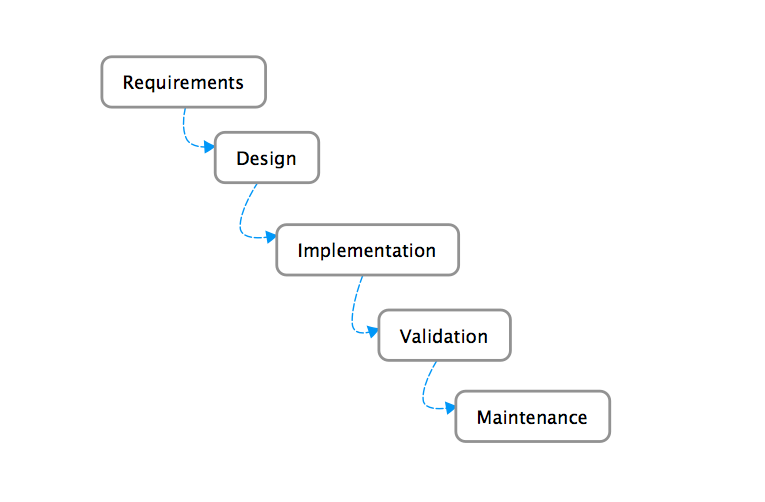
\includegraphics[width =0.8\linewidth]{WaterfallModel}}
\caption{The Waterfall Model}
\label{sec:WTF}
\label{fig:WTF}
\end{figure}

The waterfall model is a sequential design model , which has a more simple and disciplined approach. The waterfall model provides a structured development approach. It includes:
\begin{enumerate}
	\item  Requirements
	\item  Design
	\item  Implementation (Coding or construction of the project)
	\item  Validation (Testing or debugging)
	\item  Maintenance
\end{enumerate}

\subsection{Waterfall Model Life Cycle}
\paragraph{Requirements}
The requirement phase is the initial stage of the whole life cycle. At the Requirements specification phase, team will perform requirements elicitation based on the project description and the client meetings. All the selected requirements will be listed in the SRS document and implemented during the development phase.

\paragraph{Design:}
The Design phase is the phase that team members to design and establish a project plan. It is essential for the team to design all the aspects of the project carefully, since any changes made in later step will be very difficult to implement.

\paragraph{Implementation:}
Once the entire system is designed properly and completely, the main developers will start to implement the software of the project at this phase. Proper SRS documents and plans at earlier phases will be helpful. 

\paragraph{Validation:}
After the implementation is done, the QA engineers will start the Validation phase, involving testing the overall system and ensuring all requirements have being achieved. The tests include to detect whether the system is working as the previous plan.

\paragraph{Maintenance:}
After the first release of the software, the team will need to maintain the system and fix possible bugs which would be found by users.

\subsection{Advantages}
\begin{enumerate}
	\item  Simple and disciplined linear software process flow.
	\item  Well written documentation will be produced earlier in the software life cycle.
	\item  Software release to the client on deadline.
\end{enumerate}

\subsection{Disadvantages}
\begin{enumerate}
	\item  Unable to adopt change during development
	\item  Heavy documents
	\item  Late discovery of technical problems.
	\item  Can not have working software until the end of the development.
	\item  Testing is only completed at later stages of the project .

\end{enumerate}

\subsection{Minimize the Negative Impact}
The waterfall model is a one way model, which is not allowed to make much change on the later phase. In order to overcome some disadvantages and minimise the potential risk of the Waterfall Model, developers need to apply the following improvements to the Waterfall Model.

\begin{enumerate}
	\item  In order to avoid changes after the Requirements phase, the requirements stage will require well documented questions and answers from the client. Any unclear features of the project must be dealt with immediately by appropriate confirmation from the client during the client meetings.
	\item  During the design phase, all components of the system need to be properly managed and designed with the correct requirements. In this stage, developers use one Gantt chart to ensure against any setbacks to the project. It is essential to use the risk plan to avoid and fix any issues.
	\item  Documentation manager need to keep all the documents up to date, and adapt to the requirements changes.
	\item  The implementation stage should not be started until all features are well designed and negotiated by all team member. It is necessary to record all potential issues to prevent any change of from previous phase. It is also essential to release the working prototypes to the client frequently in order to gather more feedbacks from the client.  
	\item  During project validation, the system needs to be tested thoroughly. It is required to test the system by all team members, more test will be helpful to fix more bugs. 
\end{enumerate}













\chapter{Work plan}



\section{Work activities}



\subsection{Documents}
\begin{tabular}{|c|p{1cm}|p{3cm}|p{7cm}|}%{| l | l | l | l | }
\hline
\centering SerialNumber     &	Name 	&	TimeRequired		&	Description	       											\\ \hline
W000 & Poster & 2 Days & Produce a poster that show the pictures and the important
information(such as name, degree and  specialty) of the all the group members.  \\ \hline

W001		&	SRS	&	1 week	&	A Software Requirements Specification document (SRS) is produced. It defines all the details as to the requirements of the robot software and the requirements of the host software.  \\ \hline
W002		&	SPMP	&	1 week	&	Produce a Software Project Management Plan (SPMP), which provides all the information about how and who works on which aspect of the project and time arrangement. \\ \hline	
\end{tabular}
%\paragraph{W000: Poster}
%Produce a poster that show the pictures and the important information(such as name, degree and  specialty) of the all the group members.
%\paragraph{Time Required:}2 Days\\


%\paragraph{W001: SRS}
%A Software Requirements Specification document (SRS) is produced. It defines all the details as to the requirements of the robot software and the requirements of the host software.
%\paragraph{Time Required:}1 Week\\


%\paragraph{W002: SPMP}
%Produce a Software Project Management Plan (SPMP), which provides all the information about how and who works on which aspect of the project and time arrangement. 
%\paragraph{Time Required:}1 Week\\



\subsection{Robot Physical}
\begin{tabular}{|c|p{1cm}|p{3cm}|p{7cm}|}%{| l | l | l | l | }
\hline
SerialNumber     &	Name 	&	TimeRequired		&	Description	       											\\ \hline
W003		&	Robot Build		& 3 Days		& The robot must be built to complete all the tasks that are required. That is including detect all the elements, mark them on the map and auto-pilot. \\ \hline
W004		&	Robot Testing	&	1 Day	& Once the robot building is completed, it should be tested properly. These must include movement tests which tests that if the robot can moves by any directions correctly and smoothly on the map; accuracy tests which tests that if the robot can move accurately(for example if the program let the robot rotate 90 degrees, the robot should rotate exactly 90 degrees. Tests can be repeated to find small error); stability tests which aim to test that if the robot is likely to fall apart.\\ \hline	
\end{tabular}
%\paragraph{W003: Robot Physical Design\&Build}
%The robot must be built to complete all the tasks that are required. That is including detect all the elements, mark them on the map and auto-pilot.
%\paragraph{Time Required:}3 Days\\



%\paragraph{W004: Robot Testing}
%Once the robot building is completed, it should be tested properly. These must include movement tests which tests that if the robot can moves by any directions correctly and smoothly on the map; accuracy tests which tests that if the robot can move accurately(for example if the program let the robot rotate 90 degrees, the robot should rotate exactly 90 degrees. Tests can be repeated to find small error); stability tests which aim to test that if the robot is likely to fall apart.
%\paragraph{Time Required:}1 Day\\


\subsection{Host Software}
\begin{tabular}{|c|p{1cm}|p{3cm}|p{7cm}|}%{| l | l | l | l | }
\hline
SerialNumber     &	Name 	&	TimeRequired		&	Description	       											\\ \hline
W005		&	GUI	&	5 Days 	&	Produce a GUI that has map display, manual control button, battery capacity, Bluetooth status. It should be clear and easy to use. It allow user for full control over the robot.\\ \hline
W006		&   Manual Control	&	5 Days & After the robot is built correctly and fully tested, the manual control software should be developed to achieve the basic movement: move forward, move backward, turn left, turn right. The robot can be controlled with PC keyboard or GUI. \\ \hline
W007	  & Speed Control 	&	2 Days	& Add speed Control function into the GUI to allow users adjust speed while the robot is moving. \\ \hline
\end{tabular}
%\paragraph{W005: GUI}
%Produce a GUI that has map display, manual control button, battery capacity, Bluetooth status. It should be clear and easy to use. It allow user for full control over the robot.
%\paragraph{Time Required:}5 Days\\



%\paragraph{W006: Manual Control}
%After the robot is built correctly and fully tested, the manual control software should be developed to achieve the basic movement: move forward, move backward, turn left, turn right. The robot can be controlled with PC keyboard or GUI.
%\paragraph{Time Required:}5 Days\\



%\paragraph{W007: Speed Control}
%Add speed Control function into the GUI to allow users adjust speed while the robot is moving.
%\paragraph{Time Required:}2 Days\\



\subsection{Robot Software}
\begin{tabular}{|c|p{2.3cm}|p{3cm}|p{7cm}|}%{| l | l | l | l | }
\hline
SerialNumber     &	Name 	&	TimeRequired		&	Description	
								\\ \hline
W008		&	Obstacle Detection And Avoidance & 2 Weeks	& Robot can detect a obstacle in front and automatically find a path to avoid that obstacle. The robot should also mark that obstacle on the map. If the position of a obstacle is already known, the robot must avoid it and correct the position if there are errors. \\ \hline
W009  &  Hidden Wall Detection & 1 Week & Implement the function that let the robot can detect hidden walls by light sensor and mark them on map. The hidden wall is defined by different Grayscale.\\ \hline 
W010 & No-go Zone Detection And Avoidance & 1 Week & Be able to find the No-go zones and avoid them. The robot should also mark them on the map. If the position of a No-go zone is already known, the robot must avoid it and also correct the position or complete the border of that No-go zone.\\  \hline
W011 & Path Finding & 1 Week & Add a path finding algorithm to the robot, let it automatically drive itself to the destination and avoid all the obstructer. The map is assumed to be correct, but when the robot finds an element that is not correctly marked on map it should correct it and recalculate path according to the new map.\\ \hline
\end{tabular}
%\paragraph{W008: Wall Detection And Avoidance}
%Robot can detect a wall in front and automatically find a path to avoid that wall. The robot should also mark that wall on the map. If the position of a wall is already known, the robot must avoid it and correct the position if there are errors.
%\paragraph{Time Required:}2 Weeks\\


%\paragraph{W009: Hidden Wall Detection}
%Implement the function that let the robot can detect hidden walls by light sensor and mark them on map. The hidden wall is defined by different Grayscale.
%\paragraph{Time Required:}1 Week\\


%\paragraph{W010: No-go Zone Detection And Avoidance}
%Be able to find the No-go zones and avoid them. The robot should also mark them on the map. If the position of a No-go zone is already known, the robot must avoid it and also correct the position or complete the border of that No-go zone.
%\paragraph{Time Required:}1 Week\\




%\paragraph{W011: Path Finding}
%Add a path finding algorithm to the robot, let it automatically drive itself to the destination and avoid all the obstructer. The map is assumed to be correct, but when the robot finds an element that is not correctly marked on map it should correct it and recalculate path according to the new map.
%\paragraph{Time Required:}1 Week\\




\section{Milestones}
\subsection{Week1}
\paragraph{Introduction}
All the group members will be introduced and will begin reading the requirements of project.


\subsection{Week2}
\paragraph{Poster}
A poster will be made to introduce all the team members to client.

\subsection{Week3}
\paragraph{Client Meeting}
 The first meeting with client will be held this week. During the meeting everyone will be introduced to the client and may ask questions about the requirement. We should start to assemble our robot now.
 
\subsection{Week4}
\paragraph{Client Meeting}
The second client meeting will be held, and further requirements will be discussed. 

\subsection{Week5}
\paragraph{SRS}
The first draft of SRS is completed this week as well as a basic version of GUI.


\subsection{Week6}
\paragraph{Robot Movement and Bluetooth Connection}
Some basic movement function should be now achieved, such as move forward, backward and 90 degree turn. The robot should also be able connected with computer via Bluetooth.

\subsection{Week7}
\paragraph{Manual Control}
Robot movement can be fully controlled by computer 


\subsection{Week8}
\paragraph{Obstacles Location}
Robot will be able to locate Obstacles and avoid then, then mark them on the map.


\subsection{Week9}
\paragraph{Map Editor}
GUI should now be able to load map file and edit map. It can add or delete elements on the map.




\subsection{Week10}
\paragraph{Map Drawing and Auto-pilot}
Robot will fully pilot and discover the map by itself.


\subsection{Week11}
\paragraph{Error Correction and Improvement}
Tests will be run on the robot to find the error and correct them. Also if there are any improvement can be made, it should all be done at the end of this week.



\section{Schedule allocation}

\noindent \textbf{ID:} P \\
\noindent \textbf{Name:} Poster \\
\noindent \textbf{Start:} 31/07/12 \\
\noindent \textbf{End:} 3/08/12 \\
\noindent \textbf{Duration:} 4 days \\
\noindent \textbf{Task:}  Design a poster for our group, with every group member's information. Print out the poster before the due date.\\[0.5cm]

\noindent \textbf{ID:} SRS1D \\
\noindent \textbf{Name:} Software Requirements Specification 1st Draft\\
\noindent \textbf{Start:} 8/08/12 \\
\noindent \textbf{End:} 20/08/12 \\
\noindent \textbf{Duration:} 9 days \\
\noindent \textbf{Task:} Divide the SRS document into parts in the group meeting. Every group member completes the parts he assigned to.\\[0.5cm]

\noindent \textbf{ID:} SPMP1D \\
\noindent \textbf{Name:} Software Project Management Plan 1st Draft\\
\noindent \textbf{Start:} 20/08/12 \\
\noindent \textbf{End:} 3/09/12 \\
\noindent \textbf{Duration:} 10 days \\
\noindent \textbf{Task:} Divide the first SPMP draft document task into parts in the group meeting. Every group member completes the parts he assigned to.\\[0.5cm]

\noindent \textbf{ID:} SDD1D \\
\noindent \textbf{Name:} Software Design Document 1st Draft\\
\noindent \textbf{Start:} 27/08/12 \\
\noindent \textbf{End:} 14/09/12 \\
\noindent \textbf{Duration:} 15 days \\
\noindent \textbf{Task:} Divide the first SDD draft document task into parts in the group meeting. Every group member completes the pieces he assigned to.\\[0.5cm]

\noindent \textbf{ID:} TR \\
\noindent \textbf{Name:} Test Report\\
\noindent \textbf{Start:} 10/09/12 \\
\noindent \textbf{End:} 05/10/12 \\
\noindent \textbf{Duration:} 20 days \\
\noindent \textbf{Task:} Test every implemented function during these four weeks, add the test result to the test report after every testing.\\[0.5cm]

\noindent \textbf{ID:} UM \\
\noindent \textbf{Name:} User Manual \\
\noindent \textbf{Start:} 28/09/12 \\
\noindent \textbf{End:} 19/10/12 \\
\noindent \textbf{Duration:} 15 days \\
\noindent \textbf{Task:} User Manual is divided into different parts according to the robot's functions. Every group member is required to write the part of the function that he developed.\\[0.5cm]

\noindent \textbf{ID:} MN1 \\
\noindent \textbf{Name:} Milestone Negotiation 1 \\
\noindent \textbf{Start:} 13/08/12 \\
\noindent \textbf{End:} 20/8/12 \\
\noindent \textbf{Duration:} 5 days \\
\noindent \textbf{Task:} None\\[0.5cm]

\noindent \textbf{ID:} MN2 \\
\noindent \textbf{Name:} Milestone Negotiation 2 \\
\noindent \textbf{Start:} 7/09/12 \\
\noindent \textbf{End:} 14/09/12 \\
\noindent \textbf{Duration:} 5 days \\
\noindent \textbf{Task:} None\\[0.5cm]

\noindent \textbf{ID:} GUIF \\
\noindent \textbf{Name:} GUI Framework \\
\noindent \textbf{Start:} 2/08/12 \\
\noindent \textbf{End:} 7/08/12 \\
\noindent \textbf{Duration:} 3 days \\
\noindent \textbf{Task:} None\\[0.5cm]

\noindent \textbf{ID:} GUICP \\
\noindent \textbf{Name:} GUI Control Panel \\
\noindent \textbf{Start:} 2/08/12 \\
\noindent \textbf{End:} 6/08/12 \\
\noindent \textbf{Duration:} 3 days \\
\noindent \textbf{Task:} None\\[0.5cm]

\noindent \textbf{ID:} GUIMDP \\
\noindent \textbf{Name:} GUI Map Display Panel \\
\noindent \textbf{Start:} 6/08/12 \\
\noindent \textbf{End:} 7/08/12 \\
\noindent \textbf{Duration:} 1 days \\
\noindent \textbf{Task:} None\\[0.5cm]

\noindent \textbf{ID:} GUIRIP \\
\noindent \textbf{Name:} GUI Information Panel \\
\noindent \textbf{Start:} 8/08/12 \\
\noindent \textbf{End:} 10/08/12 \\
\noindent \textbf{Duration:} 2 days \\
\noindent \textbf{Task:} None\\[0.5cm]

\noindent \textbf{ID:} GUISLP \\
\noindent \textbf{Name:} GUI System Log Panel \\
\noindent \textbf{Start:} 13/08/12 \\
\noindent \textbf{End:} 14/08/12 \\
\noindent \textbf{Duration:} 1 days \\
\noindent \textbf{Task:} None\\[0.5cm]

\noindent \textbf{ID:} GUISMC \\
\noindent \textbf{Name:} GUI Settings and Mode Change \\
\noindent \textbf{Start:} 14/08/12 \\
\noindent \textbf{End:} 15/08/12 \\
\noindent \textbf{Duration:} 1 days \\
\noindent \textbf{Task:} None\\[0.5cm]

\noindent \textbf{ID:} GUIM \\
\noindent \textbf{Name:} GUI Settings and Mode Change \\
\noindent \textbf{Start:} 16/08/12 \\
\noindent \textbf{End:} 16/08/12 \\
\noindent \textbf{Duration:} 1 days \\
\noindent \textbf{Task:} None\\[0.5cm]

\noindent \textbf{ID:} BR \\
\noindent \textbf{Name:} Build Robot \\
\noindent \textbf{Start:} 1/08/12 \\
\noindent \textbf{End:} 14/08/12 \\
\noindent \textbf{Duration:} 11 days \\
\noindent \textbf{Task:} None\\[0.5cm]

\noindent \textbf{ID:} RM \\
\noindent \textbf{Name:} Robot Movement \\
\noindent \textbf{Start:} 2/08/12 \\
\noindent \textbf{End:} 17/08/12 \\
\noindent \textbf{Duration:} 11 days \\
\noindent \textbf{Task:} None\\[0.5cm]

\noindent \textbf{ID:} BC \\
\noindent \textbf{Name:} Blue-tooth Connection \\
\noindent \textbf{Start:} 16/08/12 \\
\noindent \textbf{End:} 16/08/12 \\
\noindent \textbf{Duration:} 1 days \\
\noindent \textbf{Task:} None\\[0.5cm]

\noindent \textbf{ID:} MCon \\
\noindent \textbf{Name:} Manual Control \\
\noindent \textbf{Start:} 17/08/12 \\
\noindent \textbf{End:} 20/08/12 \\
\noindent \textbf{Duration:} 1 days \\
\noindent \textbf{Task:} None\\[0.5cm]

\noindent \textbf{ID:} RMM \\
\noindent \textbf{Name:} Robot Movement Milestone \\
\noindent \textbf{Start:} 20/08/12 \\
\noindent \textbf{End:} 20/08/12 \\
\noindent \textbf{Duration:} 1 days \\
\noindent \textbf{Task:} None\\[0.5cm]

\noindent \textbf{ID:} MCre \\
\noindent \textbf{Name:} Manual Create \\
\noindent \textbf{Start:} 20/08/12 \\
\noindent \textbf{End:} 21/08/12 \\
\noindent \textbf{Duration:} 1 days \\
\noindent \textbf{Task:} None\\[0.5cm]

\noindent \textbf{ID:} MDR \\
\noindent \textbf{Name:} Map Display of Robot, Walls and Hidden Objects \\
\noindent \textbf{Start:} 24/08/12 \\
\noindent \textbf{End:} 27/08/12 \\
\noindent \textbf{Duration:} 1 days \\
\noindent \textbf{Task:} None\\[0.5cm]

\noindent \textbf{ID:} Map Display of Zone (Unexplored, Explored and No-go Zone) \\
\noindent \textbf{Name:} Manual Control \\
\noindent \textbf{Start:} 27/08/12 \\
\noindent \textbf{End:} 29/08/12 \\
\noindent \textbf{Duration:} 2 days \\
\noindent \textbf{Task:} None\\[0.5cm]

\noindent \textbf{ID:} DSL \\
\noindent \textbf{Name:} Display System Log \\
\noindent \textbf{Start:} 22/08/12 \\
\noindent \textbf{End:} 24/08/12 \\
\noindent \textbf{Duration:} 2 days \\
\noindent \textbf{Task:} None\\[0.5cm]

\noindent \textbf{ID:} HCL \\
\noindent \textbf{Name:} Handle Communications Loss \\
\noindent \textbf{Start:} 28/08/12 \\
\noindent \textbf{End:} 31/08/12 \\
\noindent \textbf{Duration:} 3 days \\
\noindent \textbf{Task:} None\\[0.5cm]

\noindent \textbf{ID:} GUIM2 \\
\noindent \textbf{Name:} GUI Milestone 2 \\
\noindent \textbf{Start:} 4/09/12 \\
\noindent \textbf{End:} 4/09/12 \\
\noindent \textbf{Duration:} 1 days \\
\noindent \textbf{Task:} None\\[0.5cm]

\noindent \textbf{ID:} AW \\
\noindent \textbf{Name:} Avoid Walls \\
\noindent \textbf{Start:} 23/08/12 \\
\noindent \textbf{End:} 7/09/12 \\
\noindent \textbf{Duration:} 11 days \\
\noindent \textbf{Task:} None\\[0.5cm]

\noindent \textbf{ID:} SRM1 \\
\noindent \textbf{Name:} Smart Robot Milestone 1 \\
\noindent \textbf{Start:} 7/09/12 \\
\noindent \textbf{End:} 7/09/12 \\
\noindent \textbf{Duration:} 1 days \\
\noindent \textbf{Task:} None\\[0.5cm]

\noindent \textbf{ID:} FHO \\
\noindent \textbf{Name:} Find Hidden Objects \\
\noindent \textbf{Start:} 7/09/12 \\
\noindent \textbf{End:} 14/09/12 \\
\noindent \textbf{Duration:} 5 days \\
\noindent \textbf{Task:} None\\[0.5cm]

\noindent \textbf{ID:} ASUA \\
\noindent \textbf{Name:} Auto Survy Unexplored Area \\
\noindent \textbf{Start:} 7/09/12 \\
\noindent \textbf{End:} 19/09/12 \\
\noindent \textbf{Duration:} 1 days \\
\noindent \textbf{Task:} None\\[0.5cm]

\noindent \textbf{ID:} SRM2 \\
\noindent \textbf{Name:} Smart Robot Milestone 2 \\
\noindent \textbf{Start:} 20/09/12 \\
\noindent \textbf{End:} 20/09/12 \\
\noindent \textbf{Duration:} 1 days \\
\noindent \textbf{Task:} None\\[0.5cm]

\noindent \textbf{ID:} DTMH \\
\noindent \textbf{Name:} Data Transfer Between Machine and Host \\
\noindent \textbf{Start:} 21/09/12 \\
\noindent \textbf{End:} 28/09/12 \\
\noindent \textbf{Duration:} 1 days \\
\noindent \textbf{Task:} None\\[0.5cm]

\noindent \textbf{ID:} XFLS \\
\noindent \textbf{Name:} XML File Load and Save \\
\noindent \textbf{Start:} 1/10/12 \\
\noindent \textbf{End:} 4/10/12 \\
\noindent \textbf{Duration:} 1 days \\
\noindent \textbf{Task:} None\\[0.5cm]

\noindent \textbf{ID:} FO \\
\noindent \textbf{Name:} Full Operation \\
\noindent \textbf{Start:} 5/10/12 \\
\noindent \textbf{End:} 19/10/12 \\
\noindent \textbf{Duration:} 10 days \\
\noindent \textbf{Task:} None\\[0.5cm]

\noindent \textbf{ID:} PM \\
\noindent \textbf{Name:} Project Milestone \\
\noindent \textbf{Start:} 22/10/12 \\
\noindent \textbf{End:} 22/10/12 \\
\noindent \textbf{Duration:} 1 days \\
\noindent \textbf{Task:} None\\[0.5cm]



\pagebreak
\section{Resource allocation}


\begin{center}
\begin{tabular}{| l | l |}
\hline
  Task ID 	& 			Name 																			\\ \hline
  P 		& 			Dawei Geng 																		\\ \hline
  SRSD1 	& 			Dawei Geng, Yufengbai, Jun Chen, Yatong Zhou, Shikai Li and Quang Khoi Nguyen 	\\ \hline
  SPMPD1 	& 			Dawei Geng, Yufengbai, Jun Chen, Yatong Zhou, Yunyao Yao 						\\ \hline
  SDDD1 	& 			Dawei Geng, Yufengbai, Yunyao Yao 												\\ \hline
  TR 		&  			Yufengbai, Yatong Zhou, Yunyao Yao 												\\ \hline
  UM  		& 			All Members  																	\\ \hline
  MN1 		& 			All Members 																	\\ \hline
  MN2 		& 			All Members 																	\\ \hline
  GUIF 		&  			Yatong Zhou                                                                     \\ \hline
  GUICP 	& 			Dawei Geng, Yatong Zhou and Shikai Li 											\\ \hline
  GUIMDP 	& 			Yatong Zhou and Shikai Li  														\\ \hline
  GUIRIP 	& 			Dawei Geng, Yatong Zhou and Shikai Li 											\\ \hline
  GUISLP 	& 			Shikai Li 																		\\ \hline
  GUISMC 	& 			Shikai Li 																		\\ \hline
  GUIM 		&  			Shikai Li 																		\\ \hline
  BR 		& 			Yunyao Yao 																		\\ \hline
  RM 		& 			Dawei Geng and Yufengbai 														\\ \hline
  BC 		& 			Dawei Geng and Yufengbai 														\\ \hline
  MCtrl 	& 			Dawei Geng and Shikai Li 														\\ \hline
  RMM 		& 			Dawei Geng and Yufengbai														\\ \hline
  MCre 		&  			Yatong Zhou, Shikai Li 															\\ \hline
  ME 		& 			Yatong Zhou, Shikai Li and Quang Khoi Nguyen 									\\ \hline
  MF 		& 			All Members                                                                     \\ \hline
  MDR 		& 			Dawei Geng, Yufengbai, Yatong Zhou, Shikai Li and Quang Khoi Nguyen				\\ \hline
  MDZ 		& 			Dawei Geng, Yufengbai, Yatong Zhou, Shikai Li and Quang Khoi Nguyen 			\\ \hline
  DSL 		& 			Dawei Geng, Yatong Zhou, Shikai Li and Quang Khoi Nguyen 						\\ \hline
  HCL 		& 			Dawei Geng, Yufengbai, Jun Chen, Yatong Zhou, Shikai Li  						\\ \hline
  GUIM2 	& 			All Members 																	\\ \hline
  SRM1 		& 			All Members 																	\\ \hline
  FHO 		& 			Dawei Geng, Yufengbai and Quang Khoi Nguyen 									\\ \hline
  ASUA 		& 			Dawei Geng, Yufengbai, Yunyao Yao, Yatong Zhou, Shikai Li and Quang Khoi Nguyen \\ \hline
  SRM2 		& 			All Members 																	\\ \hline
  XFLS 		& 			Dawei Geng, Yufengbai, Jun Chen and Quang Khoi Nguyen 							\\ \hline
  FO 		& 			All Members 																	\\ \hline
  PM 		& 			All members 																	\\ \hline
\end{tabular}
\end{center}


\pagebreak


\chapter{Supporting plans}

\section{Configuration management plan}
The configuration management plan demonstrates the basic plan about how we manage our project properly. It is important and necessary to make sure all items related to client's requirement are under control of the developers. The configuration management plan is also an approach to track the development and history of each developer's task. In our project, we mainly use the SVN control repository and File Folder for configuration management. The following is the specific explanation and structure of SVN and File Folder. 

\subsection{SVN Control Repository}
Since every developer's documents and codes are saved in SVN control repository, it is convenient to check everyone's contribution to the project by client. SVN is also working as a database which is used by developers to look up the process and modification of each one.\\ \\
Then team members are able to understand the newest version of the documents and codes as soon as possible. Each group member has right to upload, download, check and modify(include delete) the files in SVN repository.\\ \\
Here is the structure of SVN Repository:
\paragraph{1. SEP-Group13-Code:}
This folder is used to save all code related to control the robot and PC  in this project. 
\paragraph{2. SPMP draft:}
This folder is used to store all versions(except final version) of Software Project Management Plan report.

\begin{enumerate}
 	\item different versions of PDF draft
 	\item different versions of TEX draft 
\end{enumerate}

\paragraph{3. agendas}
This folder contains the agendas of the Client Meeting and Internal Meeting.

\begin{enumerate}
	\item Team-13-InternalMeeting-"times of the meeting"-Agenda.pdf
	\item Team-13-InternalMeeting-"times of the meeting"-Agenda.tex
	\item Team-13-Meeting-"times of the meeting"-Agenda.pdf
	\item Team-13-Meeting-"times of the meeting"-Agenda.tex
\end{enumerate}

\paragraph{4. code samples}
This folder is used to collect all test codes for this project.

\begin{enumerate}
	\item GUI
	\item BTRobotServer
	\item Robot Movement
	\item test-codes
\end{enumerate}

\paragraph{5. Documents}
This folder is used to store the final version of documents.
\paragraph{6. SRS draft}
This folder is used to save all versions(except final version) of Software Requirement Specification report 

\begin{enumerate}
	\item different versions of PDF draft
 	\item different versions of TEX draft 
\end{enumerate}

\paragraph{7. minutes}
This folder contains the minutes of the Client Meeting and Internal Meeting.
\begin{enumerate}
	\item Team-13-InternalMeeting-"times of the meeting"-Minutes.tex
	\item Team-13-Meeting-"times of the meeting"-Minutes.pdf
	\item Team-13-Meeting-"times of the meeting"-Minutes.tex
\end{enumerate}
\subsection{File Folder}
File Folder is used to collect all materials which is printed out(including the minutes and the agendas). The feedback and the draft documents are also saved in the file folder. By using file folder, the client is easy to understand the progress of the project and is convenient to mention more requirements for us in every meeting.\\ \\
The file folder is also used as a summary for every week in internal meeting. We use folder to record the complete part and incomplete part of the project. By this way, it is convenient for us to change the time schedule for every week.   

\section{Documentation plan}
The project requires the group to produce professional quality documentation by using LATEX. All documents should use this format and it is necessary to store all documents in pdf and tex format in SVN repository. The structure of each document is required to base on the template which is post on the CS forum. For every document, we will use "divide and merge" method, which means every document is divided to different components, each group member takes responsibility to their own part. Then each group member gives a short presentation about what they write and how they plan in every week's internal meeting.

The Required documents include:
\begin{enumerate}
	\item{\textbf{Poster} } The poster is used to demonstrate the personal information of each group member including the position and the main job of each one in this project. The client is able to use poster to understand each group member's strengths and weakness.
	\item{\textbf{Software Requirements Specification} } The purpose of these documents is to describe the tasks what need to do to reach the client's requirements. In these documents, it is also necessary to demonstrate the allocation of tasks to each group member. The client also requires analysing the potential risks and demonstrating how to avoid and solve all these risks. 
	\item{\textbf{Software Design Document} } The purpose of this report is to provide an overall architecture model of the project. In addition, we are also required to give a brief introduction on individual component task. In this document, it is necessary to use some diagrams to demonstrate the design of the whole project. 
	\item{\textbf{User Manual} } The purpose of this document is to provide a guidance and instruction sheet to the client to show them how to control this whole system. In this document, the developers need to consider that some users do not have professional knowledge related to this project.
	\item{\textbf{Group Milestones} } The milestone is used to demonstrate the progress of the project to client. For writing this document, the group members need to negotiate the working process in the internal meeting. The milestone is able to be renegotiated by discussion.
	\item{\textbf{Minutes} } The purpose of the minutes is to record the working progress and client's requirement in each meeting, The minutes are divide as client meeting minutes and internal meeting minutes. The client meeting minutes are used to record the new requirement from the client, the internal meeting minutes are used to record the content of group members' discussion.
	\item{\textbf{Agendas} } The agenda is used to schedule the process of each meeting(client meeting and internal meeting). The client is convenient to understand what hope to be demonstrated by developer in every meeting.
	\item{\textbf{Testing report} } The purpose of this document is to ensure that all students participate the testing process for the software development. Every group member is required to write a testing report to demonstrate some test case.  
\end{enumerate}
     


\section{Quality assurance plan}
\subsection{Verification and Validation process}
Each group member is required to review and check the documents and codes which are written by other group members. It is necessary to make a standard including how to write the documents and the codes. In addition, we offer the position as spell checker and code checker to check and fix every document and code to make sure the documents and codes are written as the standard. If the documents or codes is too hard to understand or do not follow the standard, the checks is able to ask the developers to rewrite the documents or codes. In internal meeting, the checkers have the responsibility to demonstrate the final version to the rest developers to do the double checking together.
\subsection{Standard}
\paragraph{Coding standard}

\begin{enumerate}
	\item When the developers build the Java Folder, the developers are required to use the function of this Java program as the folder name. For example, GUI developers are required to name the folder as GUI, the robot developers are required to name the folder as Movement or Sensor detection. In this way, other developers are convenient to find the needed Java program.
	\item The developers are required to write the developer's name, writing date and the brief explanation of this file's function on the top of each Java file. This standard is used to make the Java file clearer to be read. Meanwhile, code checkers is more convenient to check the author and the fix date.  
	\item The developers are required to write the specific comments for each method, which is convenient for others to read and save the reading time.
	\item The group members who modify others' program are required to write the name and the fix date on the bottom of the Java file. The modify part is also needed to be labeled.
	\item The standards java code and Javadoc are mainly following the oracle standards. For the specific explanation, please look up the oracle official website.
\end{enumerate}

\paragraph{Documents standard}

\begin{enumerate}
	\item The file name of each document(except minutes and agendas) is required to write in format like this: Team-13-document's name-version. The client minutes is required to write in format like this:
	Team-13-Meeting-"times of the meeting"-Minutes, the internal minutes is required to write in format like this: Team-13-InternalMeeting-"times of the meeting"-Minutes. The internal agenda is required to write in format like this: Team-13-InternalMeeting-"times of the meeting"-Agenda. The client agenda is required to write in format like this: Team-13-Meeting-"times of the meeting"-Agenda. 
	\item Each group member is required to understand how to use Latex to write the file. When developers submit the documents, it is necessary to upload both the tex and pdf file.
	\item The documents must be submitted in the correct folder. For example, the minutes have to submit in the minutes folder. It is not allowed to submit the files in the wrong folder. The developer has to make sure the documents submit in right place. 
	\item If one developer wants to delete documents, it is required to negotiate with the other group members. 
\end{enumerate}

\subsection{Testing}

\paragraph{Types of testing}
\begin{enumerate}
  	\item Development Testing: where the system is tested during development to discover bugs
and defects. Consisted of unit testing, component testing and system testing
	\item Release Testing: where a separate testing team test a complete version of the system before it is released to users.
	\item User testing: where the client test the system in their own environment. Occurs in the presentation
\end{enumerate}
\paragraph{How the test is run}
The code is tested bit by bit by JUnit to ensure that it works according to the requirement. As the software is developed, JUnit allows regression testing as the test cases is kept in an organized way.  The interface is then tested by using Abbot. The working version is expected to be available at the beginning of week 11. From that point, the build will include the tests and the automated test will be scheduled everyday. As the member develops the code, he or she has the incentive of not to break the build.   
\paragraph{Responsibilites}
Each member is responsible for unit testing his own code. As a component is usually done by more than one member, the component testing, which focus on interfaces is done by that team. Once different versions are integrated, the system testing will be done by the main developers, who include almost all the team members to detect bugs. After that, the QA engineers, which includes Khoi Nguyen, Shikai Li and Jun Chen will do the release testing and ensures that the product meets it requirement.
\paragraph{Schedule}
The testing is supposed to be completed before Monday the 22nd.
\paragraph{Test data}
The test data is generated manually by developers who try normal and exceptional scenarios. The test data is also generated by users who interact with the system.
\paragraph{Testing techniqes}
\begin{enumerate}
  \item Black-box testing (Partition Testing): Input data and output results often fall into different classes where all members of a class are related. Each of these classes is an equivalence partition or domain where the program behaves in an equivalent way for each class member.  Test cases should be chosen from each partition
	\item White-box testing (Structural Testing): use knowledge of the code to construct test cases. It has different levels of coverage, which is statement coverage (node coverage), branch coverage (edge coverage) and path coverage. White-box testing also includes mutation testing, which effectively test the tests.	
\end{enumerate}

\pagebreak


% Appendicies %
\newpage
\appendix

% Forms %
\chapter{Risk Report Forms}
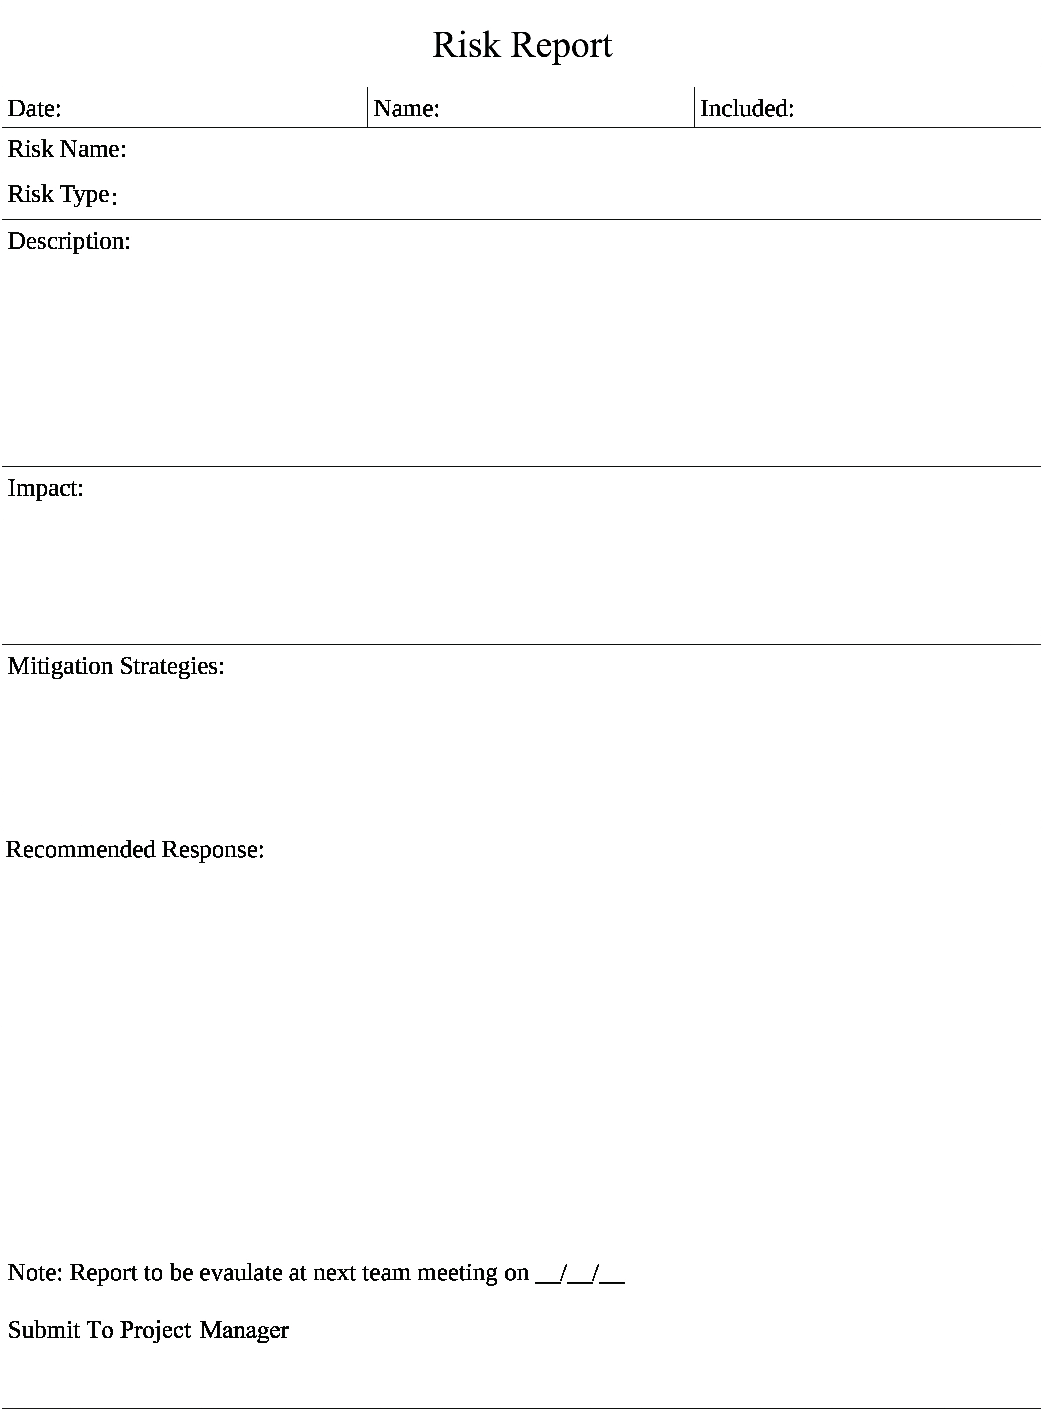
\includepdf{risk_report.pdf}
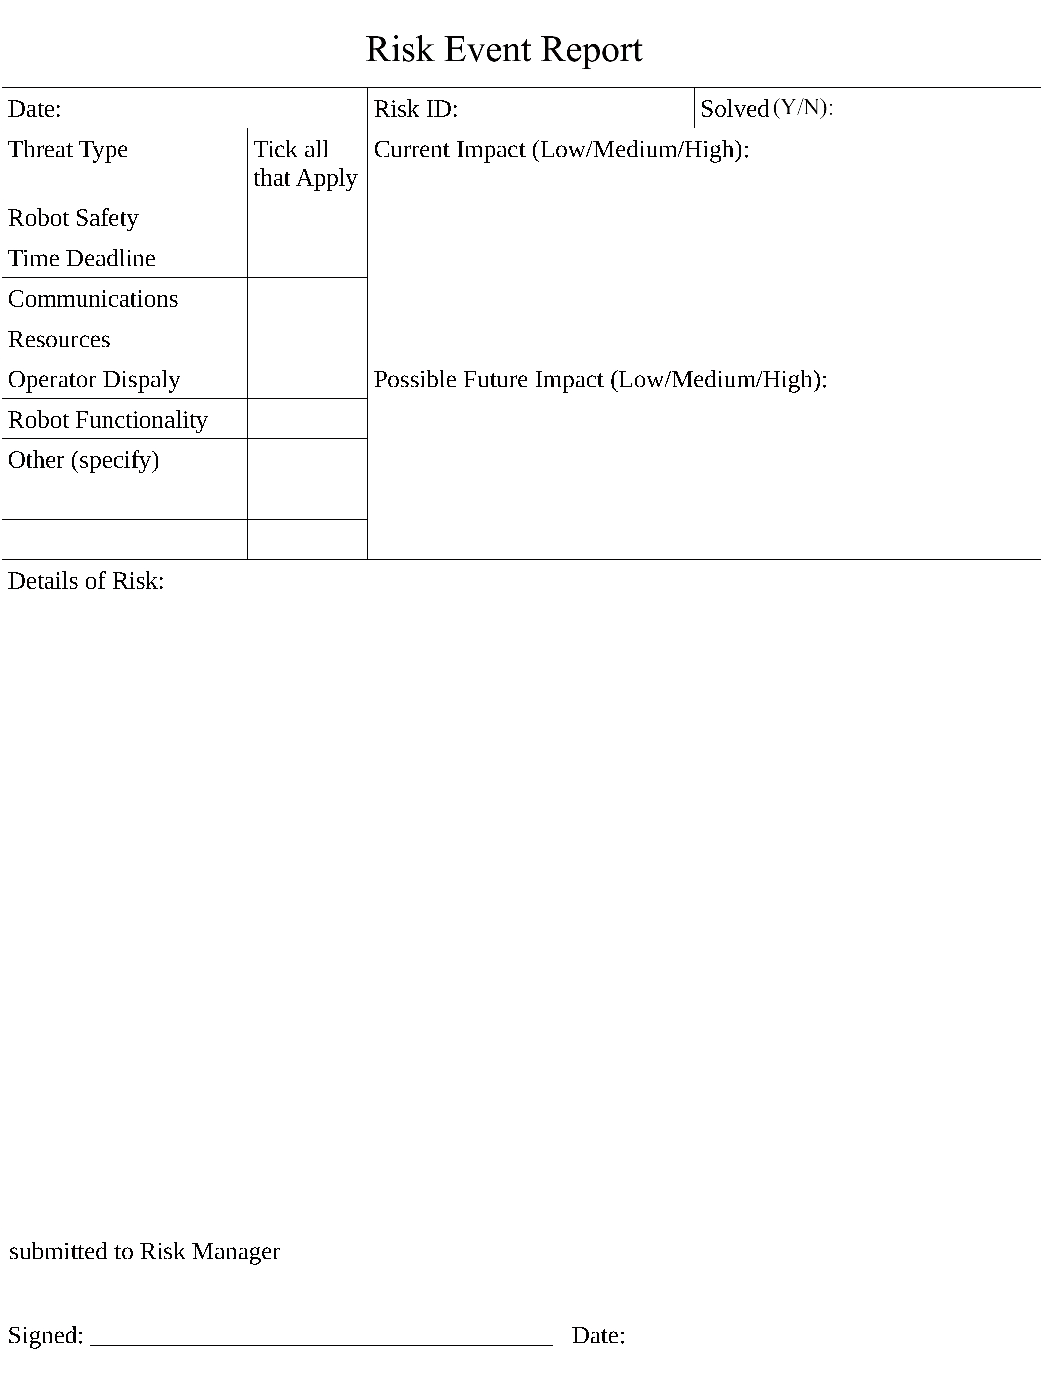
\includepdf{risk_event_report.pdf}

%Gantt Charts%
\chapter{Project Gantt Chart}
\includepdf{SEP_gantt_chart.pdf}


\chapter{Glossary}
\textbf{Automatic Mode}:  Mode of operation, completely controlled by robot and host machine, without human input of movements. \\
\\ \textbf{Bluetooth}: Wireless connection used to communicate between robot and host machine.\\
\\ \textbf{Explored Area}: The area that robot have inspected, which allows robot to travel safely.  \\
\\ \textbf{Gird}: A size of 50mm*50mm area in map, which contains 4 pixels. Each gird can be labeled as explored, unexplored, or "no go".\\
\\ \textbf{GUI}: Graphical User Interface. It displays the map panel, control panel and status panel.\\
\\ \textbf{JAR}: Java ARchive, an archive file format which is widely used by java class files.\\
\\ \textbf{JRE}: Java Runtime Environment.\\ 
\\ \textbf{Light Sensor}: Sensor used to detect hidden walls within the site, located at the front of the robot. The sensor returns the distance of the object.\\
\\ \textbf{Manual Mode}: Mode of operation. Movements controlled directly through the user.\\
\\ \textbf{Milestone}: A schedule to demonstrate the functions which need to implement before the due day\\
\\ \textbf{"no go" zone}: A zone predefined is forbidden for the robot to enter. \\
\\ \textbf{Pixel}: A size of 25mm*25mm area in map, defined as the smallest resolution, which is also the smallest area of hidden walls that robot can detect.  \\
\\ \textbf{Project Risk}: The risk list include the happened and potential risks.\\
\\ \textbf{QA}: Quality Assurance.\\
\\ \textbf{SDD}: Software Design Document.\\
\\ \textbf{SEP}: Software Engineering and Project.\\
\\ \textbf{SPMP}: Software Project Management Plan.\\
\\ \textbf{Ultrasonic Sensor}: Sensor used to detect walls and obstacles within the site, located at the front of the robot. The sensor returns the distance of the object.\\
\\ \textbf{Unexplored Area}: The area that robot have not inspected, which can be considered dangerous.  \\
\\ \textbf{Waterfall Model}: A sequential design model made up of five stages.\\
\\ \textbf{XML}: Extensible Markup Language. The map is saved as an XML file.








\end{document}
